\documentclass{article}
\usepackage{fontspec}
\usepackage[margin=1in]{geometry}
\usepackage{amsmath, amssymb}
\usepackage{xcolor}
\usepackage[most]{tcolorbox}
\usepackage{tikz}
\usepackage{pgfplots}
\pgfplotsset{compat=1.18}
\usepackage{listings}
\usepackage{booktabs}
\usepackage{colortbl}
\usepackage{algorithm}
\usepackage{algpseudocode}
\usepackage{hyperref}
\title{Class / Lecture Notes}
\author{Generated by AI Meeting Pro}
\date{\today}
\begin{document}
\maketitle
\title{Quantum Mechanics: A Brief Overview}
\author{}
\date{}
\maketitle

\section*{Core Concepts Explained}

The origins of quantum mechanics can be traced back to the atomic view of matter, which presaged the development of quantum theories. The key difference between atomic theory and quantum theory is that while atomic theory only discretizes matter, quantum theory also discretizes light and energy.

Newton is often credited with the invention of quantum mechanics, although he did not call it as such. His corpuscular view of light, which posits that light is made up of particles, was in opposition to Huygens' wave theory. The double slit experiment played a crucial role in resolving this debate, as it provided evidence for the wave-like behavior of light.

The electronic charge was first quantified in the 1800s and 1900s through the works of Faraday, Avogadro, Lockschmidt, and others. The discovery of the photon as an elementary particle was important for understanding spectroscopy and the conservation of photons in chemical reactions.

In the 1930s, a new form of quantum mechanics emerged that is still used today. This form of quantum mechanics is characterized by its strange and counterintuitive properties, such as superposition and entanglement.

\section*{Important Definitions \& Formulas}

\begin{itemize}
    \item Quantum Mechanics: A fundamental theory in physics that describes the behavior of matter and energy at the atomic and subatomic level.
    \item Corpuscular Theory: The view that light is made up of particles, proposed by Newton.
    \item Wave Theory: The view that light is a wave, proposed by Huygens.
    \item Double Slit Experiment: An experiment that demonstrates the wave-like behavior of light and electrons.
    \item Electronic Charge (e): The fundamental unit of electric charge, equal to approximately $1.602 \times 10^{-19}$ coulombs.
    \item Photon: A particle of light, with an energy proportional to its frequency.
\end{itemize}

\section*{Study Guide / Key Takeaways}

\begin{tcolorbox}[colback=blue!5!white, colframe=blue!75!black]
    \textbf{Key Points:}
    \begin{enumerate}
        \item Quantum mechanics is a fundamental theory that describes the behavior of matter and energy at the atomic and subatomic level.
        \item The origins of quantum mechanics can be traced back to the atomic view of matter, which presaged the development of quantum theories.
        \item Newton's corpuscular theory posited that light is made up of particles, while Huygens' wave theory posited that light is a wave.
        \item The double slit experiment provided evidence for the wave-like behavior of light and electrons.
        \item The electronic charge was first quantified in the 1800s and 1900s through the works of Faraday, Avogadro, Lockschmidt, and others.
        \item The discovery of the photon as an elementary particle was important for understanding spectroscopy and the conservation of photons in chemical reactions.
        \item A new form of quantum mechanics emerged in the 1930s that is still used today and is characterized by its strange and counterintuitive properties, such as superposition and entanglement.
    \end{enumerate}
\end{tcolorbox}

\begin{figure}[h]
    \centering
    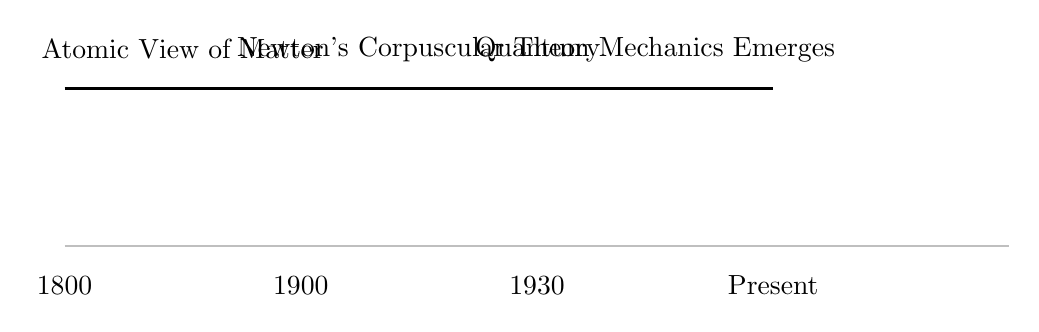
\begin{tikzpicture}
        % Timeline
        \draw[thick, gray!50] (0, 0) -- (12, 0);
        \node at (0, -0.5) {1800};
        \node at (3, -0.5) {1900};
        \node at (6, -0.5) {1930};
        \node at (9, -0.5) {Present};

        % Events
        \draw[thick] (0, 2) -- (3, 2);
        \node at (1.5, 2.5) {Atomic View of Matter};
        \draw[thick] (3, 2) -- (6, 2);
        \node at (4.5, 2.5) {Newton's Corpuscular Theory};
        \draw[thick] (6, 2) -- (9, 2);
        \node at (7.5, 2.5) {Quantum Mechanics Emerges};
    \end{tikzpicture}
    \caption{Timeline of Key Events in Quantum Mechanics}
\end{figure}

\begin{table}[h]
    \centering
    \begin{tabular}{|c|c|c|}
        \hline
        Concept & Advantage & Disadvantage \\
        \hline
        Atomic Theory & Simple to understand & Only discretizes matter \\
        \hline
        Quantum Theory & Discretizes light and energy & Strange and counterintuitive properties \\
        \hline
    \end{tabular}
    \caption{Pros and Cons of Atomic Theory and Quantum Theory}
\end{table}

\begin{table}[h]
    \centering
    \begin{tabular}{|c|c|c|}
        \hline
        Factor & Impact on Quantum Mechanics \\
        \hline
        Double Slit Experiment & Provided evidence for the wave-like behavior of light and electrons \\
        \hline
        Electronic Charge Quantification & Helped to understand the properties of matter at the atomic level \\
        \hline
        Photon Discovery & Important for understanding spectroscopy and the conservation of photons in chemical reactions \\
        \hline
    \end{tabular}
    \caption{Impact of Key Factors on Quantum Mechanics}
\end{table}

\vfill
\begin{center}
\footnotesize \textit{Generated by AI Meeting Pro on May 07, 2026 at 07:05 PM}
\end{center}

\end{document}